\documentclass{article}
\usepackage{microtype}
\usepackage{graphicx}
\usepackage{titlesec}
\usepackage{listings}
\usepackage{makecell}
\usepackage[utf8]{inputenc}
\usepackage[T1]{fontenc}

\title{Mobile Computing und Softwareengineering \\ SEN}
\author{Felix Hofinger}
\date{April 2022}

\newcommand\Tstrut{\rule{0pt}{2.6ex}}         % = `top' strut
\newcommand\Bstrut{\rule[-0.9ex]{0pt}{0pt}}   % = `bottom' strut

\setcounter{secnumdepth}{4}
\setcounter{tocdepth}{4}
\titleformat{\paragraph} 
{\normalfont\normalsize\bfseries}{\theparagraph}{1em}{}
\titlespacing*{\paragraph}
{0pt}{3.25ex plus 1ex minus .2ex}{1.5ex plus .2ex}

\begin{document}

\maketitle
\newpage
\tableofcontents
\newpage

\section{Listen}

\hfill\\
{\bf Vorteile gegenüber Arrays:}
\begin{itemize}
  \item[-] wachsen und schrumpfen
  \item[-] einfaches einfügen und löschen
\end{itemize}

\hfill\\
{\bf Nachteile gegenüber Arrays:}
\begin{itemize}
  \item[-] kein indizierter Zugriff

\end{itemize}

\subsection{Lineare List}

\begin{figure}[h!]
  \centering
  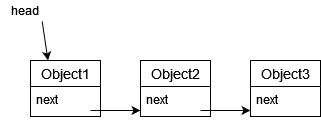
\includegraphics[scale=0.6]{list_structure.png}
  \caption{Aufbau einer Liste}
  \label{fig:list_structure}
\end{figure}

\begin{lstlisting}[language=c, tabsize=4]
struct Node {
    struct Node* next;
    int value;
}

struct List {
    struct Node* head;
}

int main() {
    struct List* list = (struct List*) malloc(sizeof(struct List));
    list->head = NULL;
}
\end{lstlisting}
\newpage

\subsubsection{Einfügen am Listen Anfang}

\begin{figure}[h!]
  \centering
  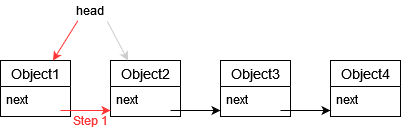
\includegraphics[scale=0.6]{list_insert_front.png}
  \caption{Einfügen am Listen Anfang}
  \label{fig:list_insert_front}
\end{figure}

\begin{lstlisting}[language=c, tabsize=4]
void prepend(struct List* list, int value) {
    struct Node* n = (struct Node*) malloc(sizeof(struct Node));
    n->value = value;
    n->next = list->head;
    list->head = n;
}
\end{lstlisting}

\subsubsection{Einfügen am Listen Ende}

\begin{figure}[h!]
  \centering
  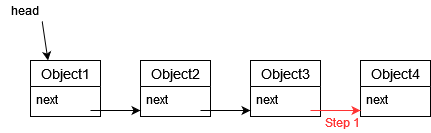
\includegraphics[scale=0.6]{list_insert_end.png}
  \caption{Einfügen am Ende der Liste}
  \label{fig:list_insert_end}
\end{figure}

\begin{lstlisting}[language=c, tabsize=4]
void append(struct List* list, int value) {
    struct Node* n = (struct Node*) malloc(sizeof(struct Node));
    n->value = value;
    n->next = NULL;
    
    if (list->head == NULL) {
        list->head = n;
        return;
    }
    
    struct Node* p = head;
    while (p->next != NULL) {
        p = p->next;
    }
    p->next = n;
}
\end{lstlisting}

\subsubsection{Suchen}

\begin{lstlisting}[language=c, tabsize=4]
struct Node* search(struct List* list, int value) {
    struct Node* p = list->head;
    while (p != NULL && p->value != value) {
        p = p->next;
    }
    return p;
}
\end{lstlisting}

\subsubsection{Löschen am Listen Anfang}

\begin{figure}[h!]
  \centering
  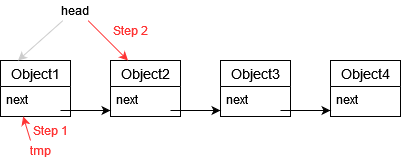
\includegraphics[scale=0.6]{list_delete_front.png}
  \caption{Löschen am Anfang der Liste}
  \label{fig:list_delete_front}
\end{figure}

\begin{lstlisting}[language=c, tabsize=4]
struct Node* remove(struct List* list) {
    if (list->head != NULL) {
        struct Node* tmp = list->head;
        list->head = list->head->next;
        free(tmp);
    }
}
\end{lstlisting}
\newpage

\subsubsection{Löschen eines Knotens mit Schlüssel}

\begin{figure}[h!]
  \centering
  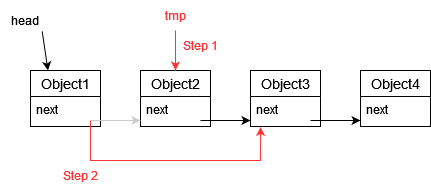
\includegraphics[scale=0.6]{list_delete.png}
  \caption{Löschen in der Mitte der Liste}
  \label{fig:list_delete}
\end{figure}

\begin{lstlisting}[language=c, tabsize=4]
void remove(struct List* list, int value) {
    struct Node* p = list->head;
    struct Node* prev = NULL;
    
    while (p != NULL && p->value != value) {
        prev = p;
        p = p->next;
    }
    
    if (p == NULL) {
        return; // Liste leer oder Wert nicht gefunden
    }
    
    if (p == list->head) {
        list->head = list->head->next;
        free(p);
    } else {
        prev->next = p->next;
        free(p);
    }
}
\end{lstlisting}

\subsubsection{Eine Liste Reversen}

\begin{lstlisting}[language=c, tabsize=4]
void reverse() {
	if (count() <= 0) return;
	node* n = head, * new_head = NULL;
	int i;
	for (i = 0; n != NULL; i++) {
		if (new_head == NULL) {
			new_head = n;
		} else {
			node* nn = n->next;
			n->next = new_head;
			new_head = n;
			n = nn;
		}
	}

	n = new_head;
	for (int j = 0; j < i; j++) {
		n = n->next;
	}
	n->next = NULL;

	head = new_head;
}
\end{lstlisting}

\subsubsection{Sortieren einer Liste}

\begin{lstlisting}[language=c, tabsize=4]
void sort() {
	int len = count();

	for (int j = 0; j < len; j++) {
		for (int i = 0; i < len - j - 1; i++) {
			node* n = head;
			for (int k = 0; k < i; k++) { 
			    n = n->next; 
			}
			
			node* npp = n->next;
			if (n->data > npp->data) {
				int temp = n->data;
				n->data = npp->data;
				npp->data = temp;
			}
		}
	}
}
\end{lstlisting}
\newpage

\subsection{Sortierte Liste}

\subsubsection{Einfügen (ohne doppelte)}

\begin{figure}[h!]
  \centering
  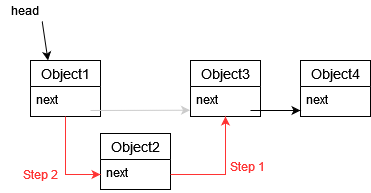
\includegraphics[scale=0.6]{list_insert.png}
  \caption{Einfügen in der Mitte einer Liste}
  \label{fig:list_insert}
\end{figure}

\begin{lstlisting}[language=c, tabsize=4]
void insert(struct List* list, int value) {
    struct Node* p = list->head;
    struct Node* prev = NULL;
    
    while (p != NULL && p->value < value) {
        prev = p;
        p = p->next;
    }
    
    if (p == NULL || p->value != value) {
        struct Node* n = (struct Node*) malloc(sizeof(struct Node));
        n->value = value;
        n->next = p;
        if (p == list->head) {
            list->head = n;
        } else {
            prev->next = n;
        }
    }
}
\end{lstlisting}
\newpage

\section{Stack}

Prinzip: LIFO (Last in, First out)

\subsection{Stack mit Array}

\begin{lstlisting}[language=c, tabsize=4]
struct Stack {
    int* data;
    int size;
    int top;
}

struct Stack* init(int stacksize) {
    struct Stack* s = (struct Stack*) malloc(sizeof(struct Stack));
    s->data = (int *) malloc(stacksize * sizeof(int));
    s->size = stacksize;
    s->top = 0;
    return s;
}

void push(struct Stack* s, int value) {
    if (s->top < s->size) {
        s->data[s->top] = value;
        s->top++;
    } else {
        exit(-1); // Stack voll!!
    }
}

int pop(struct Stack* s) {
    if (s->top > 0) {
        s->top--;
        return s->data[s->top];
    } else {
        exit(-1);
    }
}
\end{lstlisting}

\subsection{Stack mit Linked List}

\begin{lstlisting}[language=c, tabsize=4]
struct Node {
    struct Node* next;
    int data;
}

struct Stack {
    struct Node* head;
}

struct Stack* init(int stacksize) {
    struct Stack* s = (struct Stack*) malloc(sizeof(struct Stack));
    s->head = NULL;
    return s;
}

void push(struct Stack* s, int v) {
    struct Node* n = (struct Node*) malloc(sizeof(struct Node));
    n->data = value;
    n->next = s->head;
    s->head = n;
}

int pop(struct Stack* s) {
    if (s->head == NULL) {
        exit(-1);
    }
    
    int value = s->head->data;
    struct Node* n = s->head;
    s->head = s->head->next;
    free(n);
    return value;
}
\end{lstlisting}

\section{Queue}

Prinzip: FIFO (First in, First out)

\subsection{Queue als Array}

\begin{lstlisting}[language=c, tabsize=4]
typedef struct {
    int* queue;
    int head;
    int tail;
    int elements;
    int len;
} Queue;

Queue* createQueue(int startsize) {
    Queue *q = (Queue *) malloc(sizeof(Queue));
    q->data = (int *) malloc(sizeof(int) * startsize);
    q->capacity = startsize;
    q->size = 0;
    q->tail = 0;
    q->head = 0;
    return q;
}

void put(Queue *q, int v) {
    if (q->size >= q->capacity) {
        printf("Not enough capacity!\n");
        return;
    }
    q->data[q->tail] = v;
    q->size++;
    q->tail = (q->tail + 1) % q->capacity;
}

int get(Queue *q) {
    if (q->size <= 0) {
        printf("Queue empty!\n");
        return NULL;
    }
    int v = q->data[q->head];
    q->head = (q->head + 1) % q->capacity;
    return v;
}

int peek(Queue *q) {
    if(q->size > 0){
        return q->data[q->head];
    }
    printf("Queue empty\n");
    return -1;
}
\end{lstlisting}

\subsection{Queue als List}

\begin{lstlisting}[language=c, tabsize=4]
typedef struct {
    Node* next;
    int value;
} Node;

typedef struct {
    Node* head;
    Node* tail;
} Queue;

Queue* createQueue() {
    Queue* q = (Queue*) malloc(sizeof(Queue));
    q->head = NULL;
    q->tail -> NULL;
    return q;
}

void put(Queue* q, int value) {
    Node* n = (Node*) malloc(sizeof(Node));
    n->next = NULL;
    n->value = value;
    
    if (q->tail == NULL) {
        q->head = n;
        q->tail = n;
    } else {
        q->tail->next = n;
    }
}

int get(Queue* q) {
    Node* tmp = q->head;
    int v = tmp->value;
    q->head = q->head->next;
    free(tmp);
    return v;
}
\end{lstlisting}
\newpage

\section{Komplexität von Algorithmen}

TODO: add beispiel from P5b, P6f, P6b
\subsection{Beispiel}
\subsubsection{Verbesserung \#1}
\subsubsection{Verbesserung \#2}
\subsection{Analyse}
\subsection{Typische Komplexitätsfunktionen von Algorithmen}

\begin{table}[h!]
  \centering
  \begin{tabular}{ |c|c|l| }
    \hline
    1                    & konstant      & \makecell[l]{Jede Anweisung wird einmal ausgeführt. \\ Idealzustand.} \\
    \hline
    log(n)               & logarithmisch & \makecell[l]{Basis 2 ->                             \\ vierfache Datenmenge, doppelte Ressourcen} \\
    \hline
    n                    & linear        & direkt proportional                                 \\
    \hline
    n * log(n)           & n log n       & zwischen n und n²                                   \\
    \hline
    n\textsuperscript{2} & quadratisch   & \makecell[l]{wächst quadratisch                     \\ nur für kleine Probleme anwendbar} \\
    \hline
    n\textsuperscript{3} & kubisch       & \makecell[l]{wächst kubisch                         \\ nur für sehr kleine Probleme anwendbar} \\
    \hline
    2\textsuperscript{n} & exponentiell  & praktisch kaum verwendbar                           \\
    \hline
  \end{tabular}
  \caption{Komplexität von Funktionen}
  \label{tab:function_complexity}
\end{table}

\subsection{O-Notation}
TODO: add o-notation text

\subsubsection{Beispiel \#1}
\subsubsection{Beispiel \#2}

\newpage

\section{Bäume}

Jeder Knoten hat nicht nur einen, sondern mehrere direkte Nachfolger.

\begin{figure}[h!]
  \centering
  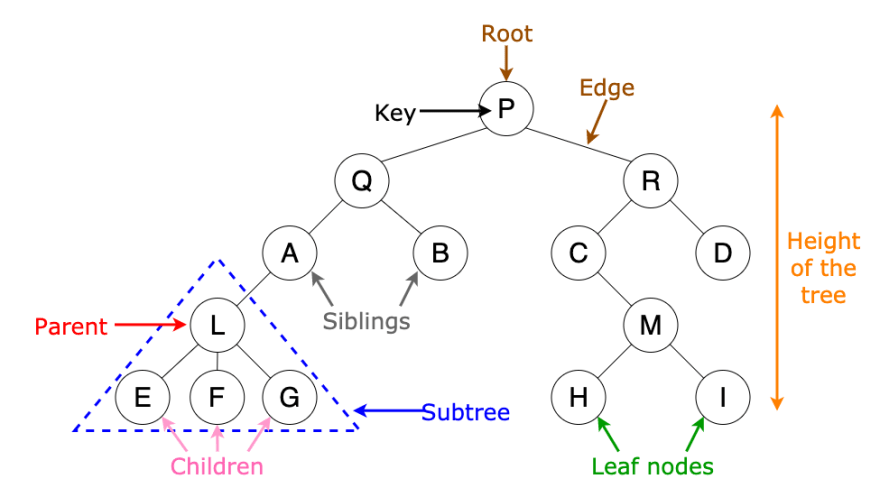
\includegraphics[scale=0.4]{tree_structure.png}
  \caption{Aufbau eines Baumes}
  \label{fig:tree_structure}
\end{figure}

\subsection{Binärbäume}

Jeder Knoten hat maximal 2 Söhne (Children).

\hfill\\
{\bf Verboten:}
\begin{itemize}
  \item[-] Zyklen
  \item[-] zwei Väter (Parents)
\end{itemize}

\subsection{Binäre Suchbäume}

\begin{lstlisting}[language=java, tabsize=4]
class Node {
    int value;
    Node left;
    Node right;
    Node(int value) {
        this.value = value;
        left = null;
        right = null;
    }
}
\end{lstlisting}
\newpage
\begin{lstlisting}[language=java, tabsize=4]
class Tree {
    Node root;
    
    Tree() {
        root = null;
    }
    
    Node search(int value) {
        ...
    }
    
    void insert(int value) {
        ...
    }
    
    Node delete(int value) {
        ...
    }
}
\end{lstlisting}

\subsubsection{Suchen}

{\bf Problemgröße}: Anzahl der Knoten bzw. Anzahl der zu durchsuchenden Werte. \\ {\bf O(log n)}: Bei 15 Knoten gibt es maximal 4 Such-Schritte.

\paragraph{Iterativ}

\begin{lstlisting}[language=java, tabsize=4]
Node search(int value) {
    Node p = root;
    while (p != null) {
        if (p.value == value) return value;
        if (value < p.value) p = p.left;
        else p = p.right;
    }
    return null; // Value not found
}
\end{lstlisting}

\paragraph{Rekursiv}

\begin{lstlisting}[language=java, tabsize=4]
Node search(int value) {
    return search(root, value);
}

static Node search(Node p, int value) {
    if (p == null || p.value == value) return p;
    else if (value < p.value) return search(p.left, value);
    else return search(p.right, value);
}
\end{lstlisting}

\subsubsection{Einfügen}

{\bf Wichtig}: Immer ganz unten als Blatt (Leaf Node) einfügen.

\paragraph{Iterativ}

\begin{lstlisting}[language=java, tabsize=4]
void insert(int value) {
    Node p = root;
    Node father = null;
    while (p != null) {
        father = p;
        if (value < p.value) p = p.left;
        else p = p.right;
    }
    
    Node n = new Node(value);
    if (father == null) {
        root = n;
    } else if (value < father.value) {
        father.left = n;
    } else {
        father.right = n;
    }
}
\end{lstlisting}

\paragraph{Rekursiv}

\begin{lstlisting}[language=java, tabsize=4]
void insert(int value) {
    root = insert(root, value);
}

static Node insert(Node p, int value) {
    if (p == null) p = new Node(value);
    else if (value < p.value) p.left = insert(p.left, value);
    else p.right = insert(p.left, value);
    return p;
}
\end{lstlisting}

\subsubsection{Löschen}

TODO: add image of the 4 different cases. P9b

\begin{lstlisting}[language=java, tabsize=4]
Node delete(int value) {
    Node father = null;
    Node p = root;
    while (p != null && p.value != value) {
        father = p;
        if (value < p.value) p = p.left;
        else p = p.right;
    }
    
    if (p != null) {
        Node x;
        if (p.right == null) {
            x = p.left;
        } else if (p.right.left == null) {
            x = p.right;
            x.left = p.left;
        } else {
            Node xf = p.right;
            x = xf.left;
            while (x.left != null) {
                xf = x;
                x = x.left;
            }
            
            xf.left = x.right;
            x.left = p.left;
            x.right = p.right;
        }
        
        if (p == root) root = x;
        else if (value < father.value) father.left = x;
        else father.right = x;
        
        p.left = null;
        p.right = null;
    }
    
    return p;
}
\end{lstlisting}
\newpage

\subsection{Traversieren von Bäumen}

TODO: add example tree. P10f

\begin{table}[h!]
  \centering
  \begin{tabular}{|c|c|c|}
    \hline
    Pre-Order           & Post-Order          & In-Order            \\
    \hline
    Wurzel/links/rechts & links/rechts/Wurzel & links/Wurzel/rechts \\
    \hline
    +*24/93             & 24*93/+             & 2*4+9/3             \\
    \hline
  \end{tabular}
  \caption{Richtungen um einen Baum zu durchlaufen.}
  \label{tab:tree_traverse_orders}
\end{table}

TODO
\subsection{Balancieren von Bäumen}
\subsubsection{Tree to Vine}
\paragraph{Beispiel}
\subsubsection{Vine to Tree}


TODO
\section{Graphen}

\subsection{Speicherdarstellung}
\subsubsection{Adjazenzliste}
\subsubsection{Adjazenzmatrix}

\subsection{Depth-First-Search (DFS)}
\subsection{Breath-First-Search (BFS)}
\subsection{Minimal-Spanning-Tree (MST)}
\subsection{Shortest Path (Dijkstra)}

\newpage
\section{Hashing}


 {\bf Motivation}:
\begin{table}[h!]
  \centering
  \begin{tabular}{l|l}
    {\bf Schlüssel} & {\bf Wert}         \\
    \hline
    "Tom"           & 0664 12345 \Tstrut \\
    "Hans"          & 0699 98765         \\
    "Paul"          & ...                \\
  \end{tabular}
  \caption{Hash-Tabellen Example}
  \label{tab:hash_table_example}
\end{table}

val = tab["Tom"] => val = tab[42]

\subsection{Hashing-Funktionen}

Abbildung von großem Wertebereich (z.B.: Menge aller Dinge) auf einen kleinen Bereich (z.B.: integer).

\subsubsection{Ziel}

\begin{itemize}
  \item[-] gleichmäßige Streuung (wenig Kollisionen)
  \item[-] einfach und schnell zu berechnen
\end{itemize}

\begin{figure}[h!]
  \centering
  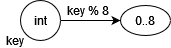
\includegraphics[scale=0.8]{hashing_easy.png}
  \caption{Einfache Hashing-Funktion}
  \label{fig:hashing_easy}
\end{figure}

\subsubsection{Langer Schlüssel (z.B.: String)}

TODO exmaple table P15f

\begin{lstlisting}[language=Java, tabsize=4]
int hash(String key) {
    int adr = 0;
    for (int i = 0; i < key.length(); i++)
        adr = (2 * adr + key.charAt(i)) % tabSize;
    return adr;
}
\end{lstlisting}

\begin{itemize}
  \item[->] sehr gute Hash-Funktion
  \item[->] ABER bei langen Schlüssel langsam
\end{itemize}

\subsubsection{Alternative}

\begin{lstlisting}[tabsize=4]
h = (key.charAt(0) * PRIMZAHL + key.charAt(key.length() - 1)
    + key.length()) % WERTEBEREICH;

hash("Anton") = (65 * 17 + 110 + 5) % 499 = 222
\end{lstlisting}

\subsection{Kollisionsstrategie}

Hashfunktion: h = str.length() \hspace{6pt} (<- sehr schlechte Hashfunktion) \Tstrut

\begin{figure}[h!]
  \centering
  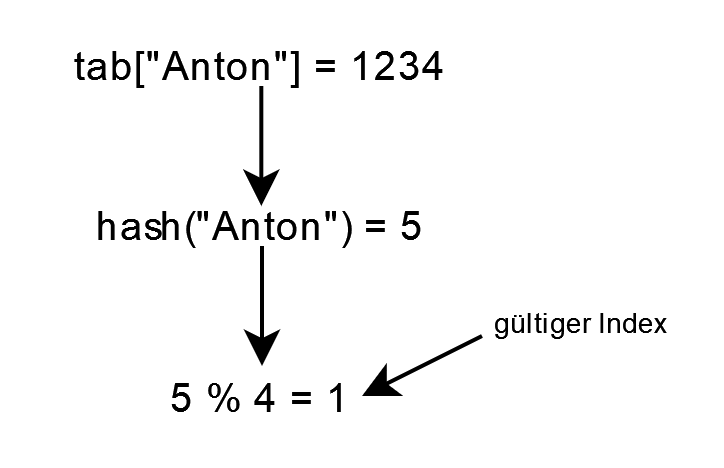
\includegraphics[scale=1.2]{hashing_procedure.png}
  \label{fig:hashing_procedure}
\end{figure}
\begin{figure}[h!]
  \centering
  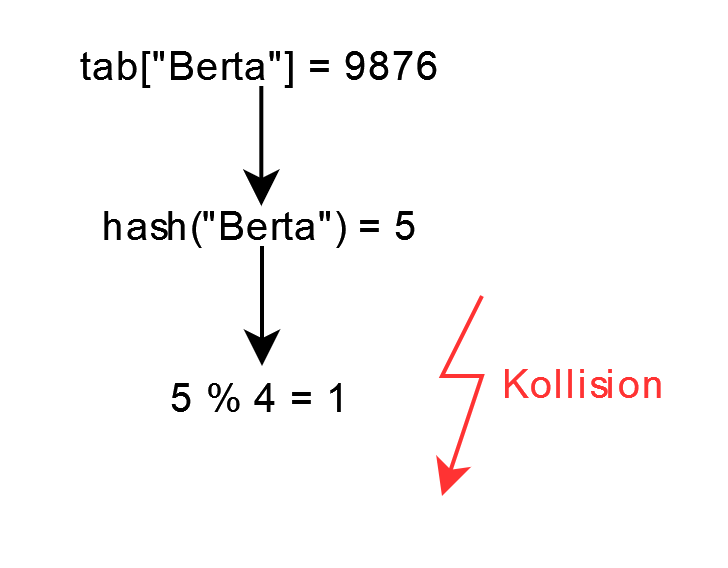
\includegraphics[scale=1.2]{hashing_collision.png}
  \label{fig:hashing_collision}
\end{figure}

\subsubsection{Seperate Chaining}
\subsubsection{Linear Probing}
\subsubsection{Quadratic Probing}


\section{Datenbanken}
\subsection{Grundsätze}
\subsection{ER-Modell}

\begin{itemize}
  \item Entity: Dinge / Gegenstände / Objekte / ... (in Java: Klassen)
  \item Relationship: Beziehung zwischen Dingen (Entities)
  \item Redundanzfreie Datenspeicherung: Information kommt nur an einer einzigen Stelle in der Datenbank vor
  \item Datenkonsitenz: Daten müssen eindeutige Informationen darstellen
\end{itemize}

\subsection{Wichtige Begriffe}

\begin{itemize}
  \item Entität (Entity): Tabellenname, Themenkreis
  \item Entitätsmenge: Datensätze
  \item Relation: Tabelle = Entität und Entitätsmenge
  \item Tuple: Datensatz
  \item Attribute: Spaltennamen
  \item Attribute-Value: Wert in einer Spalte
  \item Domain: Typ (Datentyp)
\end{itemize}

\subsection{Beziehungen}

\begin{table}[h!]
  \centering
  \begin{tabular}{ |c|l|l| }
    \hline
    1  & einfache Assoziation              & genau ein Tupel           \\
    \hline
    c  & konditionelle Assoziation         & kein oder genau ein Tupel \\
    \hline
    m  & multiple Assoziation              & mindestens ein Tupel      \\
    \hline
    mc & mutiple-konditionelle Assoziation & beliebig viele Tupel      \\
    \hline
  \end{tabular}
  \caption{Caption}
  \label{tab:my_label}
\end{table}

\subsubsection{1-1 Beziehung}
\subsubsection{1-C Beziehung}
\subsubsection{1-M Beziehung}
\subsubsection{C-C Beziehung}
\subsubsection{C-M Beziehung}


\end{document}
